\documentclass[12pt]{article}
\usepackage{polski}
\usepackage[utf8]{inputenc}
\usepackage{fullpage}
\usepackage{tabto}
\usepackage{graphicx} 
\usepackage{float}
\usepackage{caption}
\usepackage{indentfirst} 
\usepackage[table,xcdraw]{xcolor}

% zrobić macierze konfuzji
% przeczytać wnioski i chyba poprawic procenty na punkty procentowe

\linespread{1.3}
\begin{document}
%---------------------------------------------------------
%					Strona Tytułowa
%---------------------------------------------------------
\begin{titlepage}
%-----------------------Tytuł-----------------------------
\newcommand{\LINE}{\rule{\linewidth}{0.7mm}}
\center
\LINE \\[0.5cm]
\Large\textsc{Komputerowe wspomaganie diagnozowania nowotworów piersi z wykorzystaniem algorytmów minimalno-odległościowych}\\ [5mm]
\normalsize\textsc{Zastosowanie Informatyki w Medycynie}  \\[0.5cm]
\LINE \\[3cm]
%----------------------Nazwiska---------------------------
\begin{minipage}{0.5\textwidth}
\begin{flushleft} \large
\emph{Autorzy:}
		\\Mateusz Ożóg %226125
		\\Grzegorz Milaszkiewicz %226110
\end{flushleft}
\end{minipage}
~
\begin{minipage}{0.45\textwidth}
\begin{flushright} \large
\emph{Prowadzący:} \\
mgr inż. Jakub Klikowski
\end{flushright}
\end{minipage}\\[2cm]
%----------------------Stopka-----------------------------
\vfill
\center Wrocław 2019
\end{titlepage}

%---------------------------------------------------------
%					Spis treści
%---------------------------------------------------------
\newpage\thispagestyle{empty}
\mbox{}
\newpage
\renewcommand{\contentsname}{Spis treści}
\tableofcontents
\newpage
%---------------------------------------------------------
%					Część pierwsza
%---------------------------------------------------------
\section{Charakterystyka analizowanego problemu}
Tematem naszego projektu jest wspomniane w tytule, komputerowe wspomaganie diagnozowania nowotworów piersi przy pomocy algorytmów minimalno-odległościowych. Na podstawie empirycznego materiału diagnostycznego należało zbadać poprawność diagnoz losowo wybranych pacjentów dla zaimplementowanych mechanizmów rozpoznawania.
\newline
\indent Pojedyncza diagnoza przyporządkowuje pacjentkę do jednej z wyodrębnionych klas. Przeprowadzana jest na podstawie pewnych cech, które ją charakteryzują (parametry badań). Poszczególne klasy posiadają charakterystyczne wartości wyróżnionych właściwości. W procesie rozpoznawania każdy z parametrów pomaga określić przynależność do danego zbioru. Wartości niektórych z nich mogą jednoznacznie determinować klasę danego pacjenta, natomiast inne tylko ją zasugerować. W związku z tym przeprowadzono ranking cech, który posortował poszczególne parametry, zgodnie z ich znaczeniem w procesie rozpoznawania. 
\newline \indent Dla ułatwienia zrozumienia problemu i dokonania jego dokładniejszej analizy, poniżej przedstawiono krótką analizę danych poddawanych późniejszym procesom rozpoznawania.


\subsection{Analiza materiału diagnostycznego}
\indent Do badania przystąpiło 569 kobiet, u których został zdiagnozowany rak piersi. Każda z~nich została opisana za pomocą 32 wartości. Pierwsza jest numerem identyfikacyjnym, druga składa się z dwóch liter M lub B i oznacza przynależność do danej klasy.  Grupa z~rakiem łagodnym (357 kobiet) oznaczona jest literą B, natomiast z rakiem złośliwym (212 kobiet) literą M. Rozkład ilości pacjentów przynależnych do danych klas przedstawiony został na rysunku \ref{przynaleznosc_pacjentek} (malignant - nowotwór złośliwy, benign - nowotwór łagodny). Pozostałe wartości, w liczbie 30, wyznaczane były na podstawie wyglądu jądra komórkowego każdej z~pacjentek.
\newline

\begin{figure}[H]
	\centering
		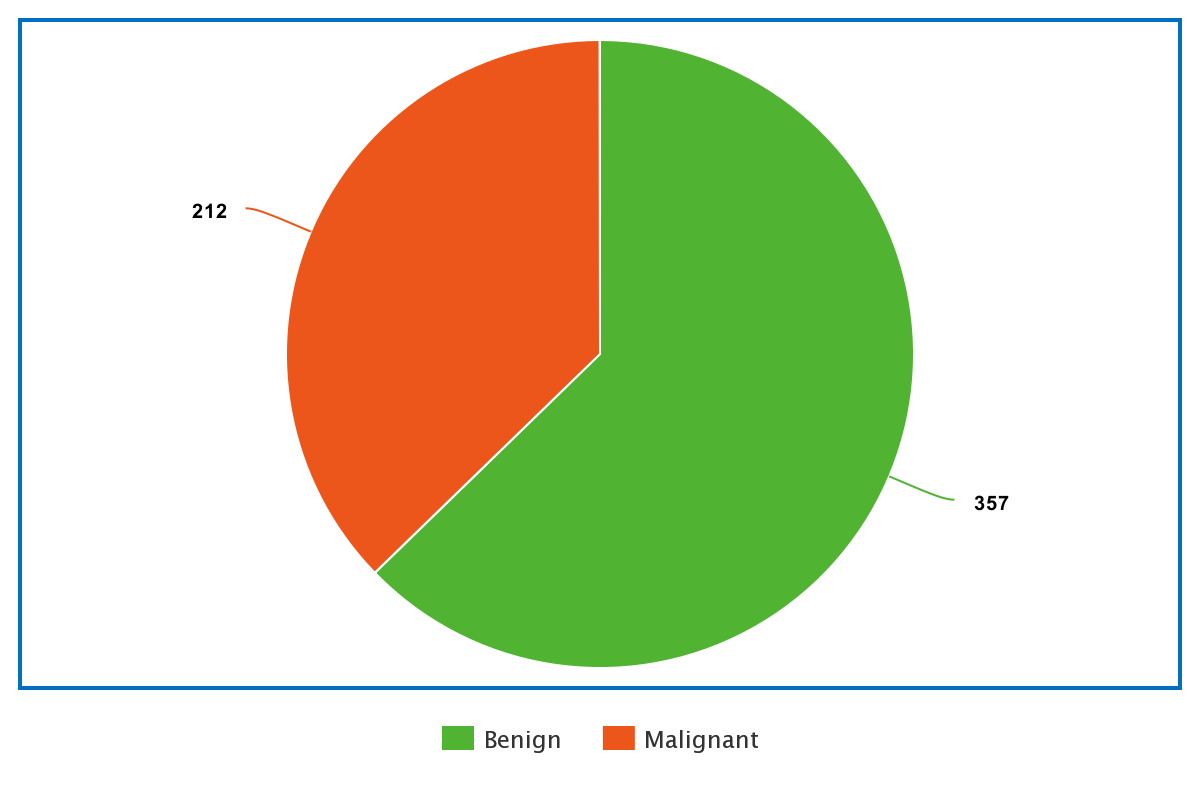
\includegraphics[scale=0.6]{images/pie_chart.png}
	\caption{Przynależność pacjentek do wyznaczonych klas}
	\label{przynaleznosc_pacjentek}
\end{figure}

\indent U każdej z kobiet zostało wyróżnionych 10 cech głównych (tabela \ref{cechy}) oraz 20 dodatkowych opisujących błąd standardowy oraz najgorszą uzyskaną wartość dla każdej z nich. Co razem daje 30 cech. 
\newline

\begin{table}[H]
\captionof{table}{Cechy jądra komórkowego wykorzystywane w procesie rozpoznawania} 
\label{cechy}
	\begin{tabular}{|p{0.2\linewidth}|p{0.74\linewidth}|}%{|l|l|}
	\hline\centering
	Numer cechy 	& Opis 				\\ \hline\centering
	1	& Promień (średnia odległość od środka do punktów na obwodzie) \\ \hline\centering
	2	& Tekstura (odchylenie standardowe wartości skali szarości) \\ \hline\centering
	3	& Obwód \\ \hline\centering
	4	& Powierzchnia \\ \hline\centering
	5	& Gładkość \\ \hline\centering
	6	& Ścisłość(obwód$^2/powierzchnia-1.0$) \\ \hline\centering
	7	& Wklęsłość (dotkliwość wklęsłych części konturu) \\ \hline\centering
	8	& Wklęsłe punkty (liczba wklęsłych części konturu) \\ \hline\centering
	9	& Symetria \\ \hline\centering
	10	& Wymiar fraktalny ("przybliżenie linii brzegowej" - 1) \\ \hline
	\end{tabular}
\end{table}
\indent Podsumowując analizę przedstawionego problemu rozpoznawania, pacjentów z grupy testowej będziemy przyporządkowywać do jednej z dwóch klas. Więcej informacji empirycznej posiadamy na temat klasy reprezentującej nowotwór łagodny, co jest spowodowane większą liczbą kobiet w jego gronie. Każda z pacjentek posiada 30 cech, które przedstawione są za pomocą wielowartościowych liczb rzeczywistych. Pojedyncza cecha z pewną dokładnością wyznacza klasyfikację do danej grupy. W celu uzyskania dokładniejszych wyników w procesie rozpoznawania będziemy przeprowadzali ranking cech, wykorzystując kryterium Kołmogorova-Smirnova, które porządkuje parametry pacjentów rozpoczynając od cech o~największym znaczeniu. Sam proces rozpoznawania opierać się będzie na implementacji klasyfikatorów minimalno-odległościowych tj. NM (nearest mean), NN (nearest neighbour) oraz KNN (k-nearest neighbours).

%---------------------------------------------------------
%					Część druga
%---------------------------------------------------------
\section{Opis stosowanych algorytmów}

\indent W procesie klasyfikacji pacjentów do poszczególnych klas zostaną wykorzystane algorytmy: najbliższej średniej oraz k-najbliższych sąsiadów. W przypadku drugiego algorytmu jako parametr k (ilość sąsiadów) zostaną przyjęte następujące wartości: 1 (najbliższy sąsiad), 5~oraz 9. Pacjentów będziemy dzielić na 2 grupy. Zbiór uczący będzie określał obiekty z zdiagnozowaną klasą. W zbiorze testowym natomiast będą znajdowali się pacjenci poddawani klasyfikacji na podstawie przetworzonych danych z grupy uczącej. Struktura danych w obu algorytmach jest identyczna. Każdy pacjent będzie określany za pomocą wektora cech tak jak to przedstawiono we wzorze poniżej.
\begin{center}
\[ \vec{X} = (x_1, x_2, ... , x_n)\]
\end{center}


Każdy zbiór będzie składał się z m takich wektorów, gdzie m oznacza liczbę przypisanych do niego pacjentów. Litera y oznacza przynależność do jednej z wyszczególnionych klas dla i-tego pacjenta (litera 'M' bądź 'B').
Zbiory uczące i testujące będą wyglądały następująco:
\begin{center}
\[ Z=\{(\vec{X_{1}}, y_{1}), (\vec{X_{2}}, y_{2}), ... , (\vec{X_{m}}, y_{m})\}\]
\end{center}

\subsection{Algorytm najbliższej średniej}
\indent Algorytm polega na wyliczeniu obiektu centralnego dla każdej klasy, który jest uśrednionym wektorem uwzględniającym wszystkie próbki ze zbioru uczącego należące do danej klasy. Na jego podstawie liczona jest odległość od obiektu testowego, na którym przeprowadzana jest klasyfikacja. Obiekt ten opisany jest za pomocą poniższego wzoru.
\begin{center}
$ \vec{U_{l}}=\frac{1}{C_{l}}\sum_{i\in{C_{l}}}\vec{X_{l}} $ \cite{bib1}
\end{center}

Litera l we wzorze powyżej jest zbiorem naszych klas, natomiast $ C_{l} $ jest zbiorem indeksów próbek należących do klasy l. Klasyfikacja polega na znalezieniu najmniejszej odległości pomiędzy jednym z wektorów średnich a testowaną próbką. Klasyfikator ten możemy opisać wzorem poniżej, gdzie T jest wektorem cech niesklasyfikowanego pacjenta, a y klasą do której zostanie przypisany. 
\begin{center}
$ y=argmin_{l\in{Y}}||\vec{U_{l}}-\vec{T}|| $ \cite{bib1}
\end{center}
\indent Aby lepiej zobrazować działanie algorytmu na rysunku \ref{algorytm_nm} przedstawiony zostanie prosty przykład bazujący na próbkach umieszczonych w przestrzeni dwuwymiarowej. \newline
\begin{figure}[H]
	\centering
		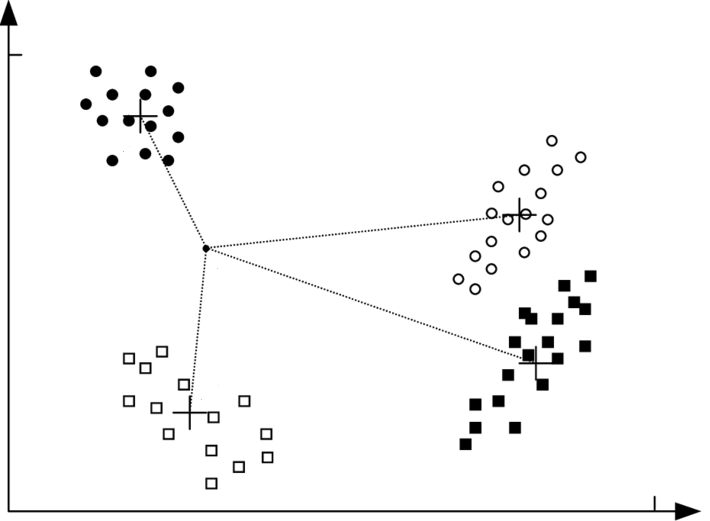
\includegraphics[scale=0.9]{images/nm_example.png}
	\caption{Przykład działania algorytmu k najbliższych sąsiadów \cite{bib2}}
	\label{algorytm_nm}
\end{figure}

 
\indent Dla każdej klasy wyznaczany jest punkt średni, na podstawie którego dokonywana będzie klasyfikacja próbki testującej (czarny punkt w centrum). Przerywane linie oznaczają drogę do centroida kolejnej klasy. 

\subsection{Algorytm k-najbliższych sąsiadów}
\indent Polega na znalezieniu k najbardziej podobnych próbek w zbiorze uczącym do obiektu testowego. Współczynnik k określa ilu sąsiadów będziemy szukać. Dla algorytmu najbliższego sąsiada wartość ta będzie równa 1. Po ustaleniu sąsiedztwa (zbiór k punktów leżących najbliżej) sprawdzamy, z której klasy danych próbek jest najwięcej. Podobieństwo obiektów badane jest przy pomocy wybranych metryk odległościowych. Dla lepszego zobrazowania działania algorytmu, poniżej znajduje się prosty przykład bazujący na wektorach w przestrzeni dwuwymiarowej. \newline
\begin{figure}[H]
	\centering
		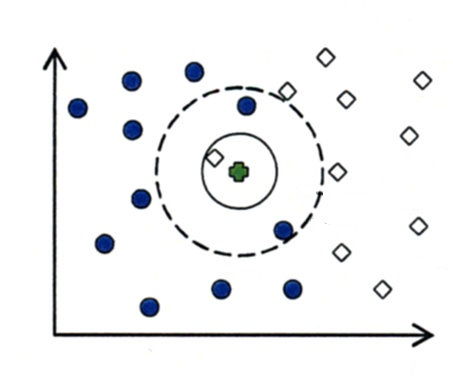
\includegraphics[scale=1]{images/knn_example.png}
	\caption{Przykład działania algorytmu k najbliższych sąsiadów \cite{bib3}}
\end{figure}

\indent Jak można zauważyć na przykładzie, klasyfikacja dla wartości parametru k równej 1 będzie przypisywała nasz obiekt testowy do klasy białej, natomiast zwiększając wielkość sąsiędztwa sytuacja się zmieni.
%---------------------------------------------------------
%					Część Trzecia
%---------------------------------------------------------
\section{Informacja o środowisku implementacyjnym}

\indent Badania zostały przeprowadzone przy pomocy języka Python w wersji 3.6. Do stworzenia rankingu cech przy użyciu kryterium Kołmogorova-Smirnova, dla każdego z parametru została użyta metoda ks\_2samp z biblioteki scipy, przyjmująca dwa wektory opisujące poszczególne klasy. Algorytmy natomiast zostały zaimplementowane z użyciem biblioteki sklearn wykorzystując metody KNeighborsClassifier oraz NearestCentroid zwracające wybrany klasyfikator. Na jego podstawie trenowany był zbiór uczący przy pomocy metody fit, a następnie przy pomocy funkcji predict przyjmującej jako parametr zbiór testowy dokonywana była diagnoza. Otrzymane wartości klasyfikacji porównano z rzeczywistym stanem badanego obiektu wykorzystując opisane w kolejnej części metryki klasyfikacji.


%---------------------------------------------------------
%					Część czwarta
%---------------------------------------------------------
\section{Opis badań eksperymentalnych}
\indent W badaniu zostały porównane algorytmy opisane w punkcie 2 niniejszej pracy. Dodatkowo każdy z nich został uruchomiony z różnymi parametrami wejściowymi tj. rodzaj metryki klasyfikacji, sposób mierzenia odległości pomiędzy próbkami, normalizacja wektora cech, jego długość czy w przypadku algorytmu najbliższego sąsiada wielkość parametru k. Porównanie różnych wariantów tych wartości zostało umieszczone w kolejnym punkcie tej pracy. Poniżej przedstawiono szczegóły dotyczące przeprowadzonych badań.\\

\subsection{Parametry klasyfikacji}
W tabeli \ref{parametry_klasyfiacji} zostały przedstawione parametry wejściowe wykorzystywane w procesie klasyfikacji.
\begin{table}[H]
\captionof{table}{Parametry klasyfikacji} 
\label{parametry_klasyfiacji}
	\begin{tabular}{|p{0.3\linewidth}|p{0.64\linewidth}|}%{|l|l|}
	\hline\centering
	Rodzaj parametru 	& Testowane wartości 		\\ \hline\centering
	Metryki klasyfikacji	& accuracy, balanced, cohen kappa \\ \hline\centering
	Algorytm	& NM, 1-NN, 5-NN, 9-NN \\ \hline\centering
	Metryka odległości	& euklides, manhatan \\ \hline\centering
	Wektor cech	& z normalizacją, bez normalizacji \\ \hline\centering
	Liczba cech	& Liczby naturalne z przedziału $<1;30>$ \\ \hline
	\end{tabular}
\end{table}

\centerline{\textbf{Opis wykorzystanych metryk klasyfikacji \cite{bib4}: }}
Podczas omawiania metryk, do lepszego zrozumienia ich działania wprowadzony został przykład, który przeliczany jest dla każdej z metryk. Funkcje te, do wyznaczenia dokładności działania klasyfikatora wykorzystują jako pierwszy parametr zbiór etykiet zgodny ze~stanem rzeczywistym  obiektów ($y_{true}$) oraz zbiór przewidywanych klas przypisywanych przez klasyfikator ($y_{pred}$). Poniżej znajdują się przykładowe oba zbiory wykorzystane w dalszych rozważaniach. \\
\begin{center}
$ y_{true} = [A, B, A, A, B, A]$ \\
$ y_{pred} = [A, B, A, A, A, B]$ \\
\end{center}
\textbf{Accuracy} - porównuje przewidywane wartości klasyfikacji z ich rzeczywistym stanem, diagnoza jest zgodna tylko w przypadku dokładnie przewidzianego wyniku. W naszym przykładzie, składającym się z 6 obiektów, 4 klasyfikator przypisał prawidłowo. W związku z tym jego dokładność przy pomocy tej metryki będzie wynosiła w przybliżeniu 0,66.
\begin{center}
$ score_{accuracy} = 0,(66) $
\end{center}
\textbf{Balanced} - metryka wykorzystywana przy niezbalansowanych zbiorach danych. Jest zdefiniowana jako średnia poprawnych wyników uzyskana dla poszczególnych klas. W przykładzie powyżej mamy dwie klasy A (4 obiekty) i B (2 obiekty). Do klasy A poprawnie zaklasyfikowano 3  obiekty, co daje nam wynik poprawności 0,75 natomiast dla klasy B jedną próbkę w~związku z tym poprawność wynosi 0,5. Ogólny wynik klasyfikatory jest średnią uzyskanych wyników:
\begin{center}
$ score_{balanced} = \frac{0,5+0,75}{2} = 0,625 $
\end{center}
\textbf{Cohen kappa} - ogólnie jest to metryka, która porównuje zgodność wyników różnych stron tzw. sędziów (oceniających przynależność do danej klasy). W naszym przypadku będzie opierała się ona o macierz konfuzji inaczej pomyłek. Jest ona narzędziem stosowanym do oceny jakości klasyfikacji. Polega na zestawieniu otrzymanych wyników z rzeczywistością w formie tabeli. Dla naszego dwu klasowego problemu rozpoznawania rozpatrywanego w~niniejszej pracy będzie miała ona kształt:

\begin{table}[H]
\begin{center}
\captionof{table}{Macierz konfuzji} 
\begin{LARGE}

\begin{tabular}{cccll}
\cline{1-3}
\multicolumn{1}{|c|}{}                          & \multicolumn{1}{c|}{\cellcolor[HTML]{FCFF2F}{\color[HTML]{333333} B}} & \multicolumn{1}{c|}{\cellcolor[HTML]{FCFF2F}{\color[HTML]{333333} M}} &  &  \\ \cline{1-3}
\multicolumn{1}{|c|}{\cellcolor[HTML]{34FF34}B} & \multicolumn{1}{c|}{$T_{b}$}                                               & \multicolumn{1}{c|}{$F_{b}$}                                               &  &  \\ \cline{1-3}
\multicolumn{1}{|c|}{\cellcolor[HTML]{34FF34}M} & \multicolumn{1}{c|}{$F_{m}$}                                               & \multicolumn{1}{c|}{$T_{m}$}                                               &  &  \\ \cline{1-3}
                                                &                                                                       &                                                                       &  & 
\end{tabular}
\end{LARGE}
\end{center}
\end{table}

Zielonym kolorem oznaczone są etykiety mówiące o rzeczywistej klasie, natomiast żółty przedstawia etykiety wyników klasyfikacji. Liczby na przekątnej oznaczają prawidłowe przypisanie do klasy. Tm oznacza prawidłowe przypisane próbek do klasy raka złośliwego, Fm natomiast nieprawidłowe przypisanie obiektów z klasy złośliwej do klasy raka łagodnego. Podobnie sytuacja wygląda w przypadku klasy B. W przypadku naszego przykładu znajdującego się w tym punkcie powyżej, macierz wraz z uzupełnionymi wartościami wygląda następująco.

\begin{table}[H]
\begin{center}
\captionof{table}{Przykładowa macierz konfuzji} 
\begin{LARGE}
\begin{tabular}{l|l|l|}
\cline{2-3}
                        & A & B \\ \hline
\multicolumn{1}{|l|}{A} & 3 & 1 \\ \hline
\multicolumn{1}{|l|}{B} & 1 & 1 \\ \hline
\end{tabular}
\end{LARGE}
\end{center}
\end{table}

Do obliczenia współczynniku dokładności metryki Cohen kappa wykorzystywany jest następujący wzór.
\begin{center}
$ k = \frac{p_{0}-p_{e}}{1-p_{e}}$ \\
\end{center}

I tak $p_{0}$ jest prawdopodobieństwem poprawnie przypisanych obiektów, w tym przykładzie było ich 4, co daje ułamek 0,(66). Natomiast $p_{e}$ składa się z prawdopodobieństwa przypisania do klasy A przez obie strony (sędziów, w naszym przypadku klasyfikatora i rzeczywistości). Wynik tego działania znajduje się poniżej wraz z obliczoną poprawnością.
\begin{center}
$ p_{e} = p_{A} + p_{B} $ \\
$ p_{A} = \frac{4}{6} * \frac{4}{6} = \frac{4}{9}$ \\
$ p_{B} = \frac{2}{6} * \frac{2}{6} = \frac{1}{9}$ \\
$ p_{e} = \frac{5}{9} $ \\

$ k = \frac{\frac{2}{3}-\frac{5}{9}}{1 - \frac{5}{9}} = \frac{\frac{1}{9}}{\frac{4}{9}} = 0,25 $ \\
\end{center}

\indent Pozostałe parametry klasyfikacji zostały wyjaśnione we wcześniejszych rozważaniach pracy bądź zostały pominięte przez autorów pracy w związku z ich małym stopniem skomplikowania.
\newline
\subsection{Badania}
\indent  Przeprowadzenie badań odbyło się z wykorzystaniem 5 razy powtarzanej metody 2-krotnej walidacji krzyżowej. Wszystkich pacjentów losowo podzielono na wspominany zbiór uczący oraz testujący. Następnie uruchomiono na testowanych obiektach poszczególne algorytmy zmieniając kolejno wyżej wymienione rodzaje parametrów. Dodatkowo zmieniano liczbę cech w wektorze opisującym próbki od wartości 1 aż do 26 (4 próbki odpadły po wykonaniu rankingu cech). Dla każdej konfiguracji zapisano wyniki. Po wykonanych badaniach zamieniono zbiory. Zbiór uczący stał się testującym i na odwrót, zbiór testujący uczącym. Po raz kolejny wykonano badania a wyniki zapisano. Proces ten, rozpoczynający się od losowania zbioru powtórzono pięciokrotnie, co sprawiło, że osiągnięte wyniki będą bardziej wiarygodne.
\newline
\indent W związku z dużą liczbą danych wynikających z ilością zmiennych parametrów, badania nie są przeprowadzone dla wszystkich możliwych konfiguracji (zmniejszyłaby się czytelność i utrudniłoby to analizę wyników). Najpierw przeprowadzone zostało porównanie metryk sprawdzających poprawność diagnoz, biorąc pod uwagę wszystkie zaimplementowane algorytmy. Następnie dla najskuteczniejszej metryki przetestowano algorytmy, sprawdzając osiągane przez nie dokładności. Dla najlepszej konfiguracji wspomnianych wyżej parametrów porównano zostały metryki odległości, a na koniec przyrównano wyniki osiągane z normalizacją wektora cech poszczególnych pacjentów oraz bez normalizacji. Osiągnięte rezultaty oraz wnioski z nich wynikające przedstawiono w dalszej części pracy.
\newpage

%---------------------------------------------------------
%					Część piąta
%---------------------------------------------------------
\section{Wyniki}
Wyniki zostały przedstawione w formie tabel, wykresów oraz macierzy konfuzji (omówione zagadnienie w punkcie wyżej). W tabelach zaznaczono kolorem zielonym komórki, które oznaczają najlepsze wyniki dla danej konfiguracji algorytmu. Dodatkowo, w związku z wielokrotnymi pomiarami oraz ich uśrednianiem zostały policzone odchylenia standardowe dla każdej z komórek. Tabela  \ref{glowna_tabela} przedstawia uśrednione wyniki wszystkich pomiarów dla różnorakich parametrów wejściowych. Jest ona wyjściowym punktem do dalszych obliczeń. Wywnioskowano z niej, który z algorytmów jest najefektywniejszy i to on został wykorzystany w dalszych rozważaniach co wspominane jest w punkcie 4 niniejszej pracy.  Odchylenia standardowe w niej zostały przedstawione w nawiasach okrągłych przy poszczególnych wynikach. \\
\indent W kolejnych podpunktach tego rozdziału będziemy mogli znaleźć następujące informacje: \\
- w podpunkcie 1 znajdziemy porównanie metryk klasyfikacji dla algorytmu 9-NN. Dodatkowo został on podzielony na 2 części w zależności od metryki odległości. Pozwala to nam na porównanie wpływu normalizacji wektora cech na wyniki dla każdej z metryk osobno.\\
- w podpunkcie 2 porównano dokładność klasyfikatorów minimalno-odległościowych. Z tabeli \ref{glowna_tabela} możemy odczytać wiele informacji na ten temat jednak w tym punkcie pracy będziemy mogli prześledzić bardziej szczegółowe badania.\\
- w przedostatnim punkcie umieszczono tabelę i wykres porównujący bezpośrednio metryki odległościowe i wpływ normalizacji wektora cech.\\
- w ostatnim punkcie przedstawiono przykładowe macierze konfuzji dla wybranych parametrów wejściowych algorytmów.
\newpage 
\begin{figure}[H]
	\centering
	\captionof{table}{Wyniki pomiarowe wykonane na podstawie zaimplementowanych algorytmów}
	\label{glowna_tabela}
		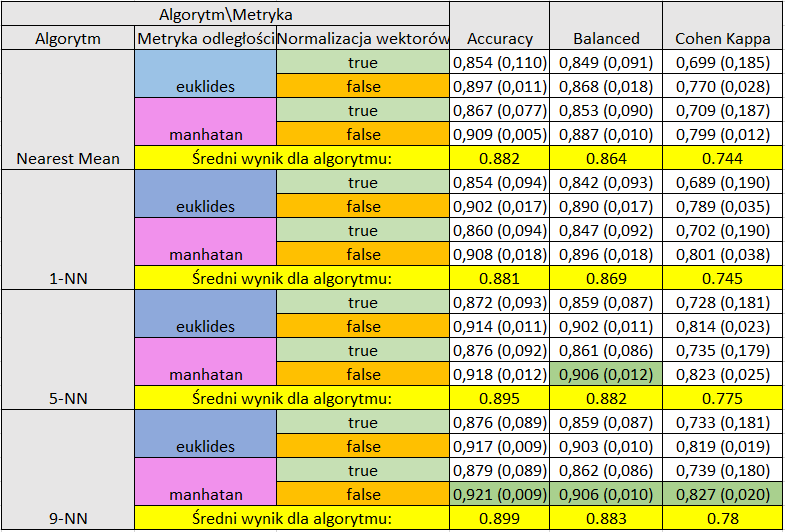
\includegraphics[scale=0.75]{images/ogolna_tabela.png}
\end{figure}

% Porownanie metryk 

%-------------------------EUKLIDES--------------------------
\subsection{Porównanie metryk klasyfikacji}
\indent Jak wspomniane było już wcześniej porównane zostały trzy wybrane metryki dla algorytmu 9-NN, wykorzystując dwie rodzaje metryk odległości oraz stosując normalizację wektora cech.
\subsubsection{Euklides}
\begin{figure}[H]
	\centering
	\captionof{table}{Porównanie metryk dla algorytmu 9-NN z normalizacją wektorów}
	\label{metryki_euklides_norm_tab}
		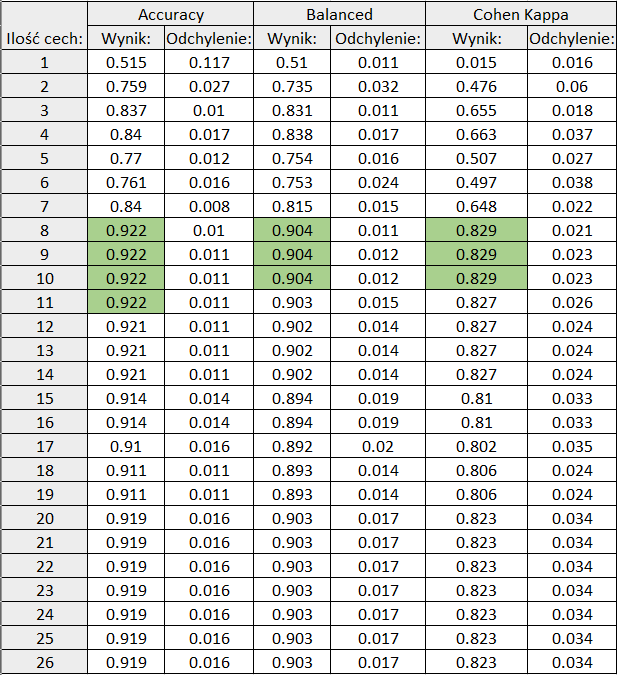
\includegraphics[scale=0.9]{images/metrics/9nn_euklides_norm_tab.png}
\end{figure}
\begin{figure}[H]
	\centering
	\captionof{table}{Porównanie metryk dla algorytmu 9-NN bez normalizacji wektorów}
	\label{metryki_euklides_bnorm_tab}
		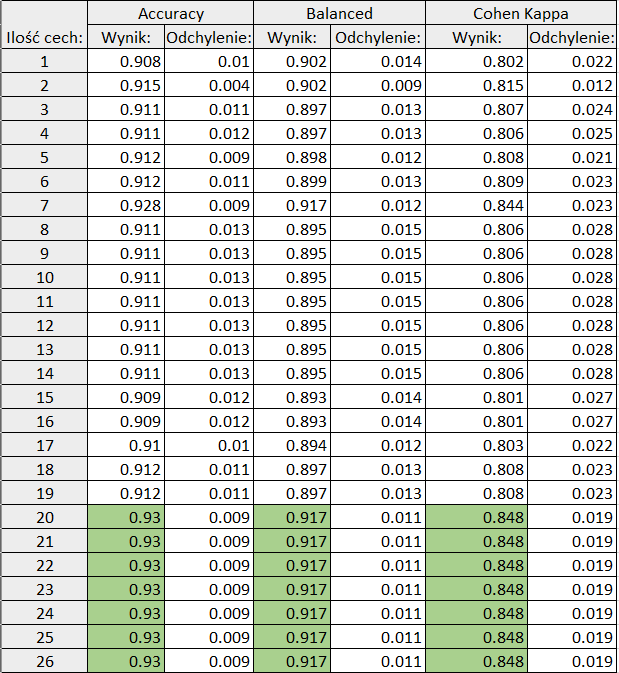
\includegraphics[scale=0.9]{images/metrics/9nn_euklides_beznorm_tab.png}
	
\end{figure}

\begin{figure}[H]
	\centering
		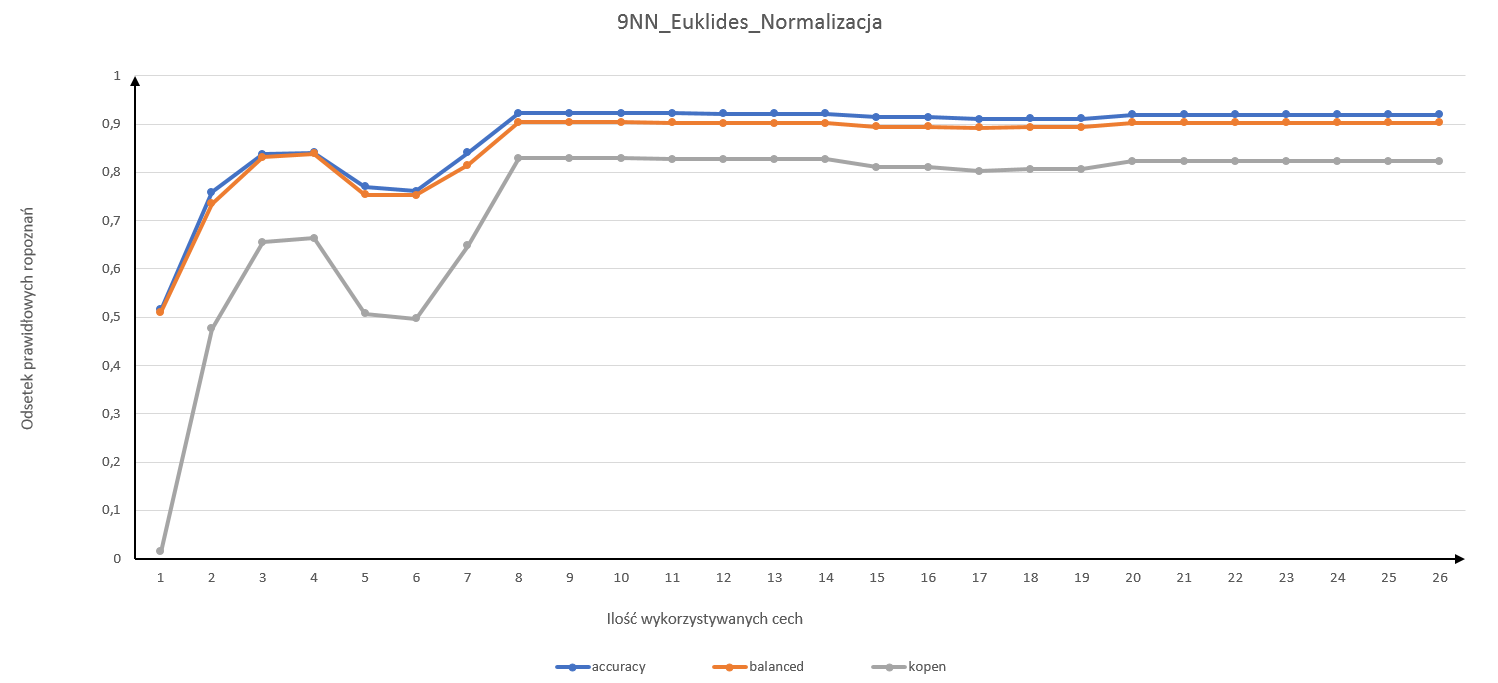
\includegraphics[scale=0.66]{images/metrics/9nn_euklides_norm.png}
	\caption{Porównanie metryk dla algorytmu 9-NN z normalizacją wektorów}
	\label{metryki_euklides_norm_wyk}
\end{figure}
\begin{figure}[H]
	\centering
		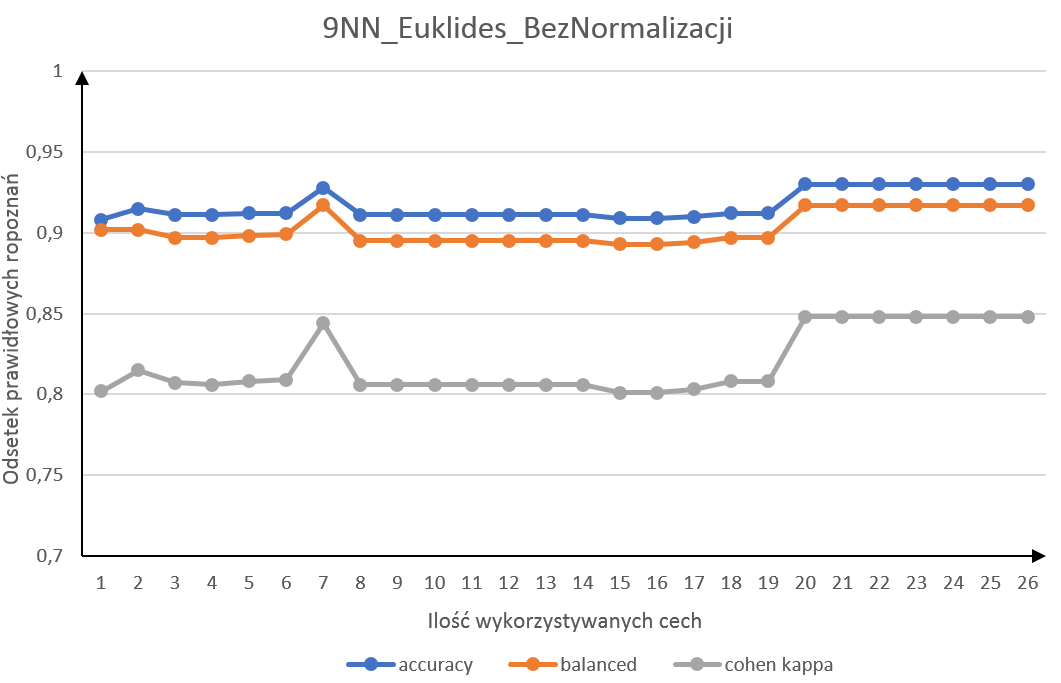
\includegraphics[scale=0.66]{images/metrics/9nn_euklides_beznorm.png}
	\caption{Porównanie metryk dla algorytmu 9-NN bez normalizacji wektorów}
	\label{metryki_euklides_bnorm_wyk}
\end{figure}
%-------------------------EUKLIDES--------------------------

\subsubsection{Manhatan}
%-------------------------MANHATAN--------------------------
\begin{figure}[H]
	\centering
	\captionof{table}{Porównanie metryk dla algorytmu 9 najbliższych sąsiadów z normalizacją wektorów}
		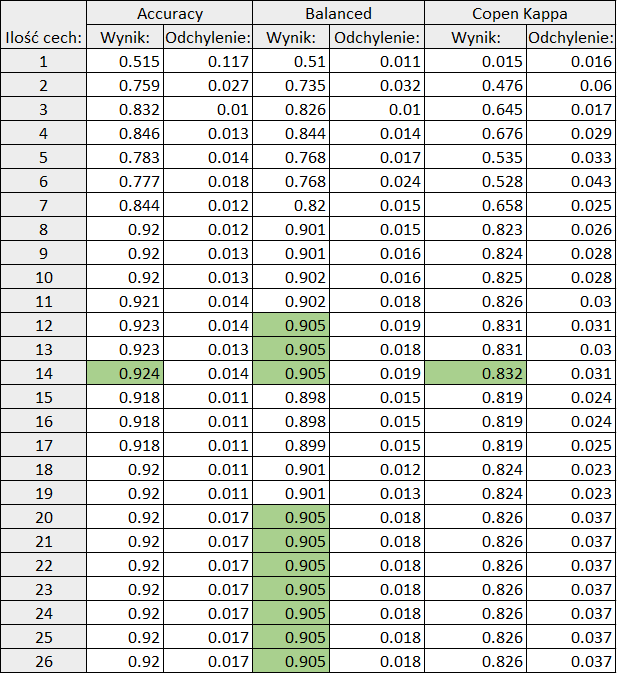
\includegraphics[scale=0.9]{images/metrics/9nn_manhatan_norm_tab.png}
	\label{metryki_manhatan_norm_tab}
\end{figure}
\begin{figure}[H]
	\centering
	\captionof{table}{Porównanie metryk dla algorytmu 9 najbliższych sąsiadów bez normalizacji wektorów}
	\label{metryki_manhatan_bnorm_tab}
		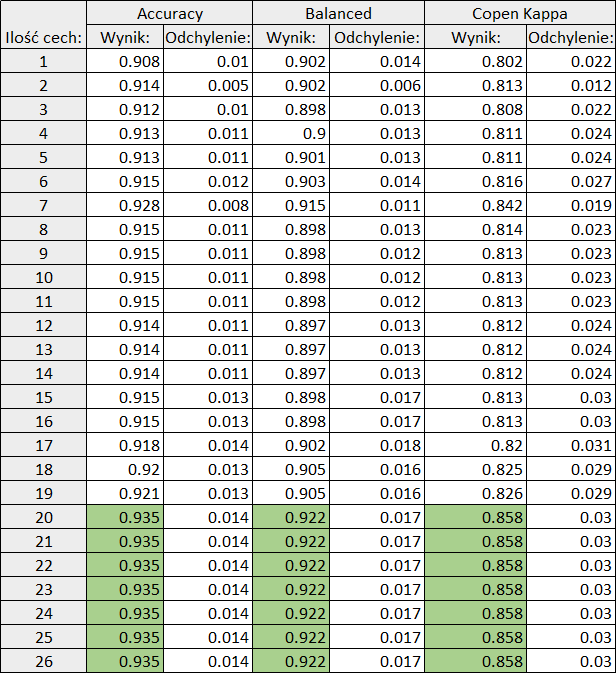
\includegraphics[scale=0.9]{images/metrics/9nn_manhatan_beznorm_tab.png}
	
\end{figure}
\begin{figure}[H]
	\centering
		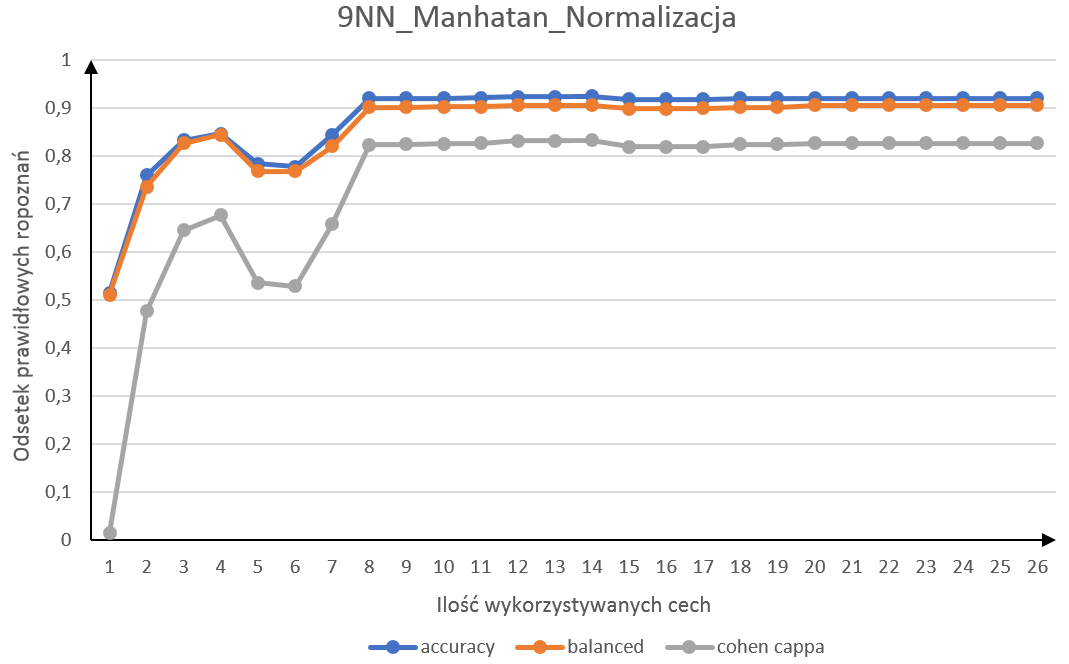
\includegraphics[scale=0.66]{images/metrics/9nn_manhatan_norm.png}
	\caption{Porównanie metryk dla algorytmu 9-NN z normalizacją wektorów}
	\label{metryki_manhatan_norm_wyk}
\end{figure}
\begin{figure}[H]
	\centering
		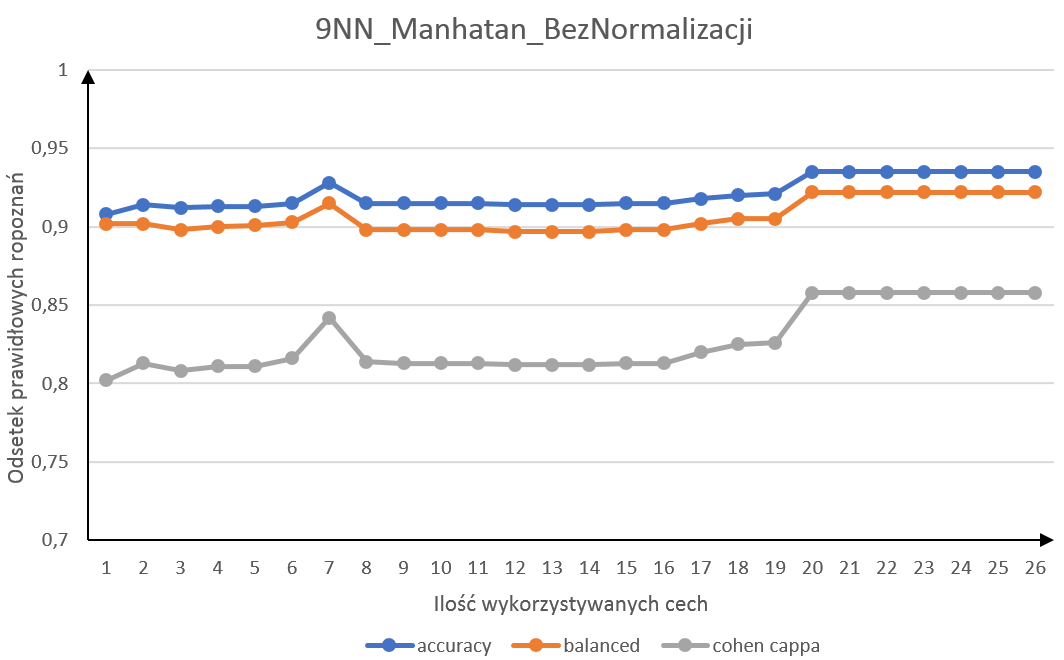
\includegraphics[scale=0.66]{images/metrics/9nn_manhatan_beznorm.png}
	\caption{Porównanie metryk dla algorytmu 9-NN bez normalizacji wektorów}
	\label{metryki_manhatan_bnorm_wyk}
\end{figure}
%-------------------------MANHATAN--------------------------
\subsection{Porównanie algorytmów}
%Porownanie algorytmów
\indent Dla metryki dającej najlepsze wyniki (accuracy) zostały porównane kolejne algorytmy minimalno-odległościowe.
\begin{figure}[H]
	\centering
	\captionof{table}{Porównanie algorytmów dla metryki odległościowej \textit{Euklides} z normalizacją wektorów}
	\label{algorytmy_euklides_norm_tab}
		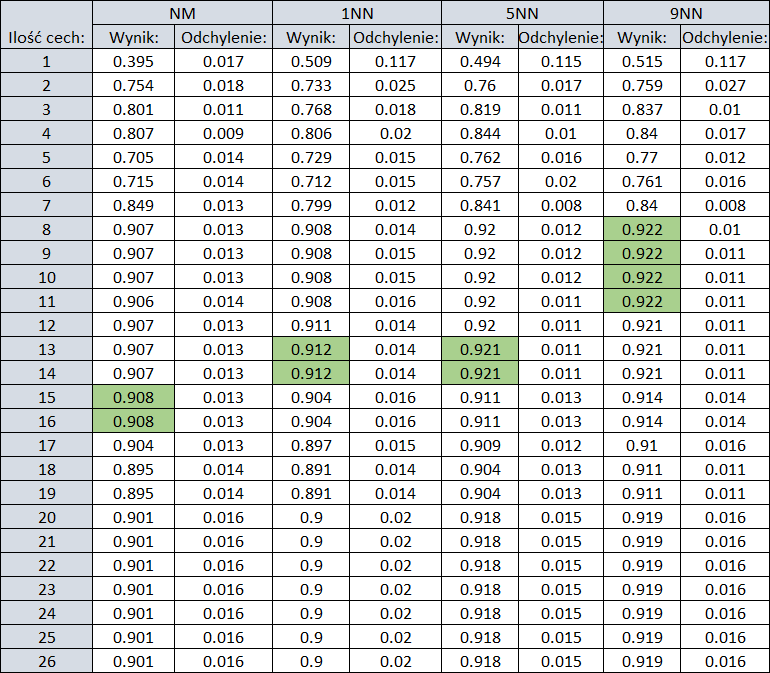
\includegraphics[scale=0.8]{images/algorithms/euklides_norm_tab.png}
	
\end{figure}

\begin{figure}[H]
	\centering
	\captionof{table}{Porównanie algorytmów dla metryki odległościowej \textit{Manhatan} z normalizacją wektorów}
	\label{algorytmy_manhatan_norm_tab}
		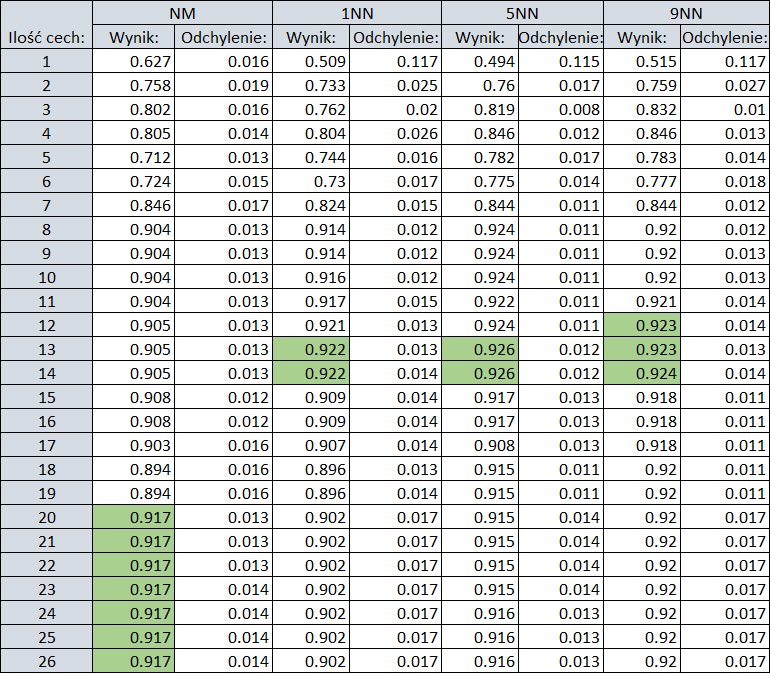
\includegraphics[scale=0.8]{images/algorithms/manhatan_norm_tab.png}
	
\end{figure}

\begin{figure}[H]
	\centering
		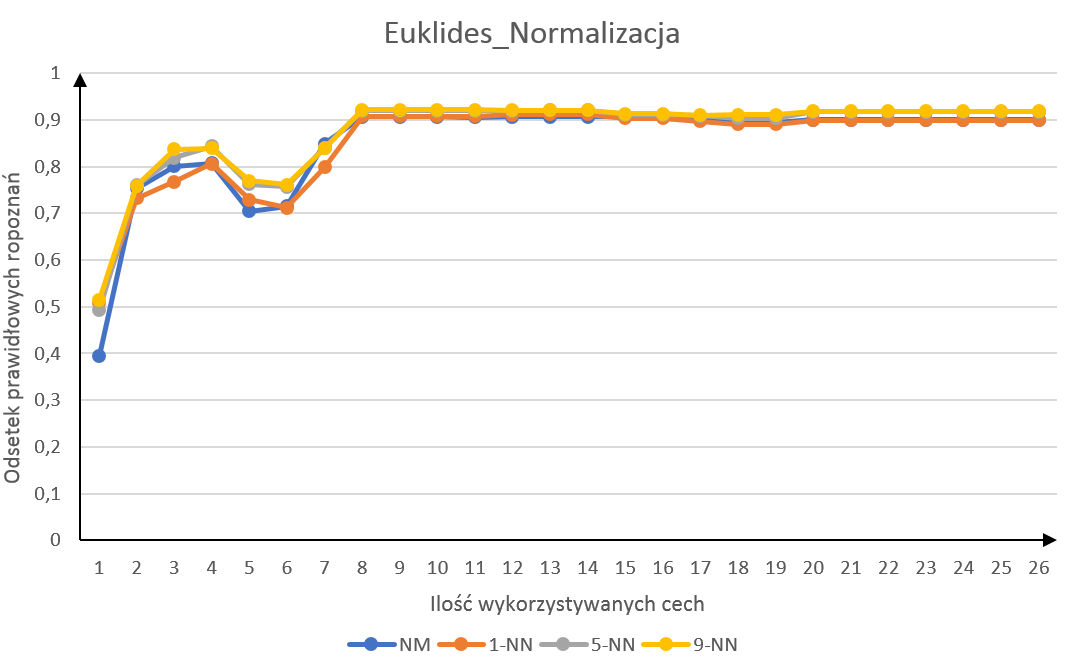
\includegraphics[scale=0.66]{images/algorithms/euklides_norm.png}
	\caption{Porównanie algorytmów dla odległości \textit{Euklides} z normalizacją wektorów}
	\label{algorytmy_euklides_norm_wyk}
\end{figure}

\begin{figure}[H]
	\centering
		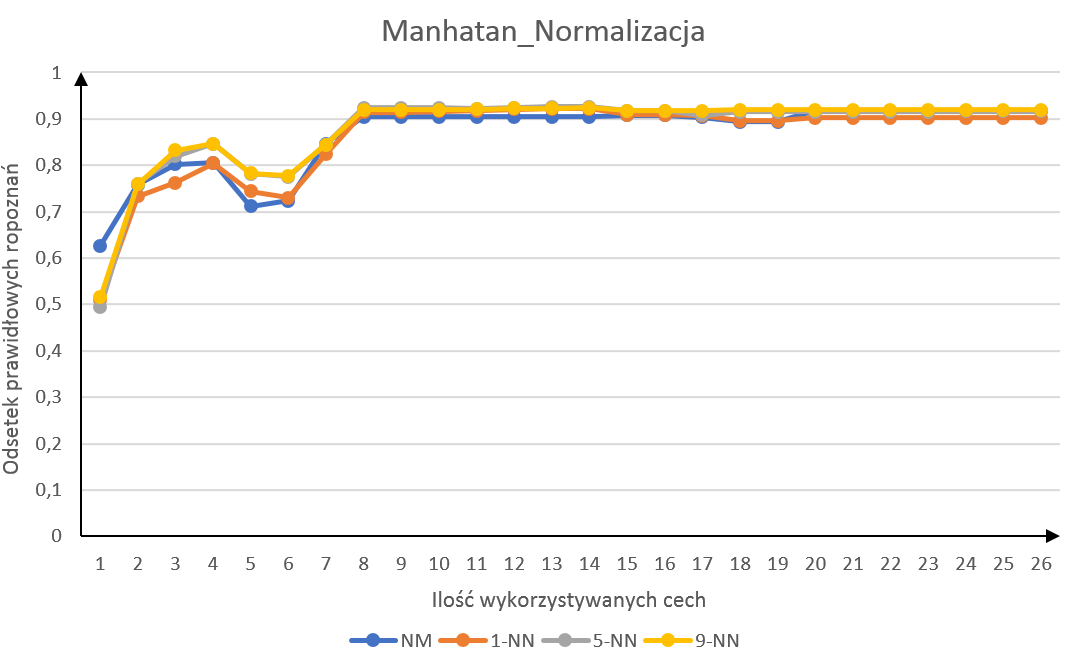
\includegraphics[scale=0.66]{images/algorithms/manhatan_norm.png}
	\caption{Porównanie algorytmów dla odległości \textit{Manhatan} z normalizacją wektorów}
	\label{algorytmy_manhatan_norm_wyk}
\end{figure}

\begin{figure}[H]
	\centering
	\captionof{table}{Porównanie algorytmów dla metryki odległościowej \textit{Euklides} bez normalizacji}
	\label{algorytmy_euklides_bnorm_tab}
		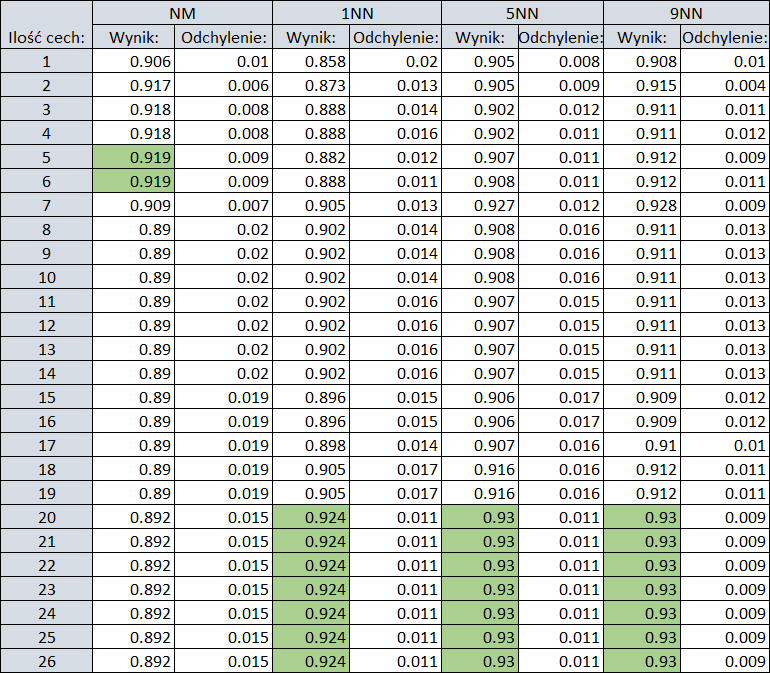
\includegraphics[scale=0.8]{images/algorithms/euklides_beznorm_tab.png}
\end{figure}
	
\begin{figure}[H]
	\centering
	\captionof{table}{Porównanie algorytmów dla metryki odległościowej \textit{Manhatan} bez normalizacji}
	\label{algorytmy_manhatan_bnorm_tab}
		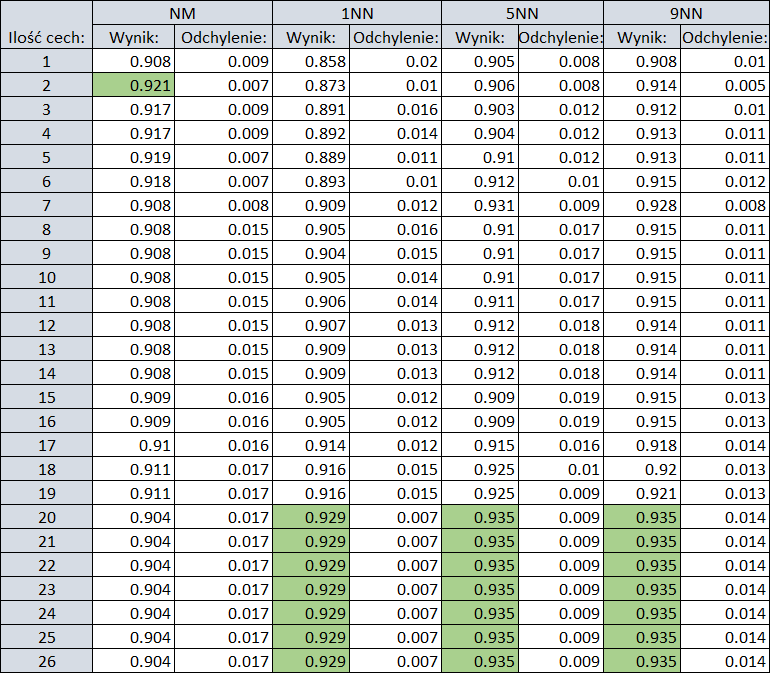
\includegraphics[scale=0.8]{images/algorithms/manhatan_beznorm_tab.png}
	
\end{figure}


\begin{figure}[H]
	\centering
		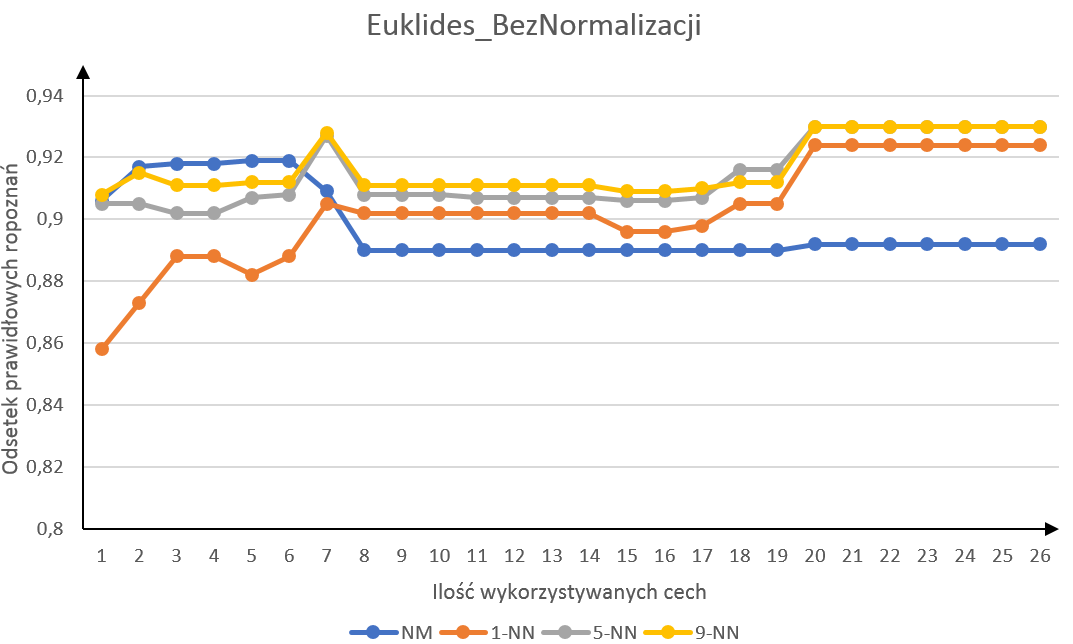
\includegraphics[scale=0.66]{images/algorithms/euklides_beznorm.png}
	\caption{Porównanie algorytmów dla odległości \textit{Euklides} bez normalizacji wektorów}
	\label{algorytmy_euklides_bnorm_wyk}
\end{figure}


\begin{figure}[H]
	\centering
		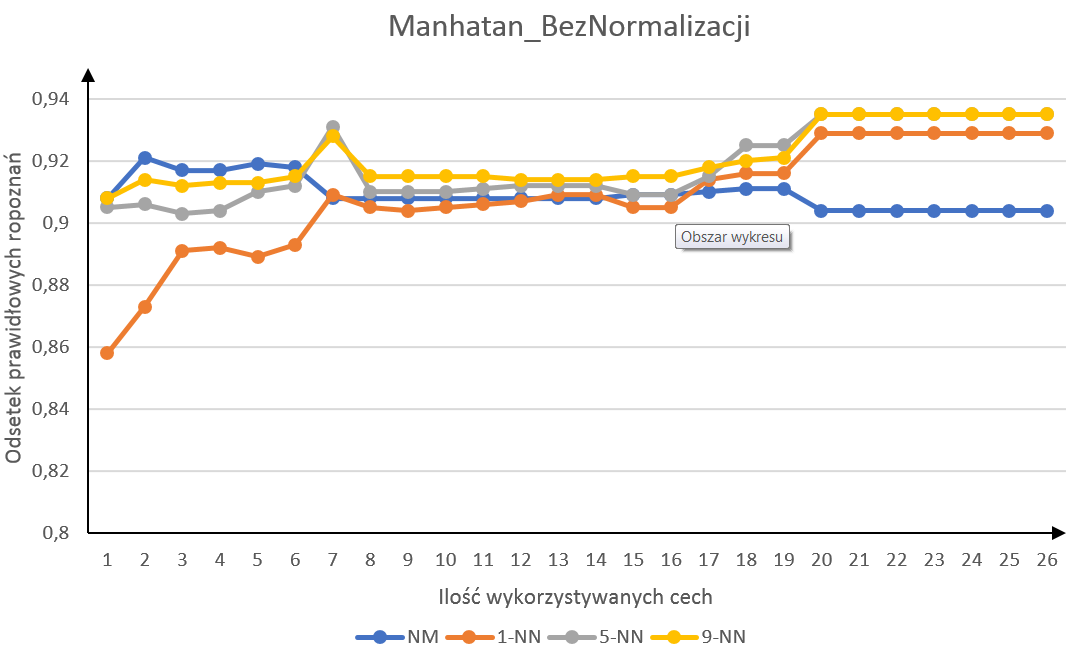
\includegraphics[scale=0.66]{images/algorithms/manhatan_beznorm.png}
	\caption{Porównanie algorytmów dla odległości \textit{Manhatan} bez normalizacji}
	\label{algorytmy_manhatan_bnorm_wyk}
\end{figure}


% Porównanie metryk odległościowych
\subsection{Porównanie metryk odległościowych}
\indent Dla algorytmu 9-NN i metryki accuracy uruchomione zostały algorytmy w zależności od metryki odległości oraz normalizacji wektora cech. Na wykresie (rysunek \ref{odleglosci_wyk}) możemy dokonać ich porównania.
\begin{figure}[H]
	\centering
	\captionof{table}{Porównanie metryk odległościowych i reprezentacji wektorów cech}
	\label{odleglosci_tab}
		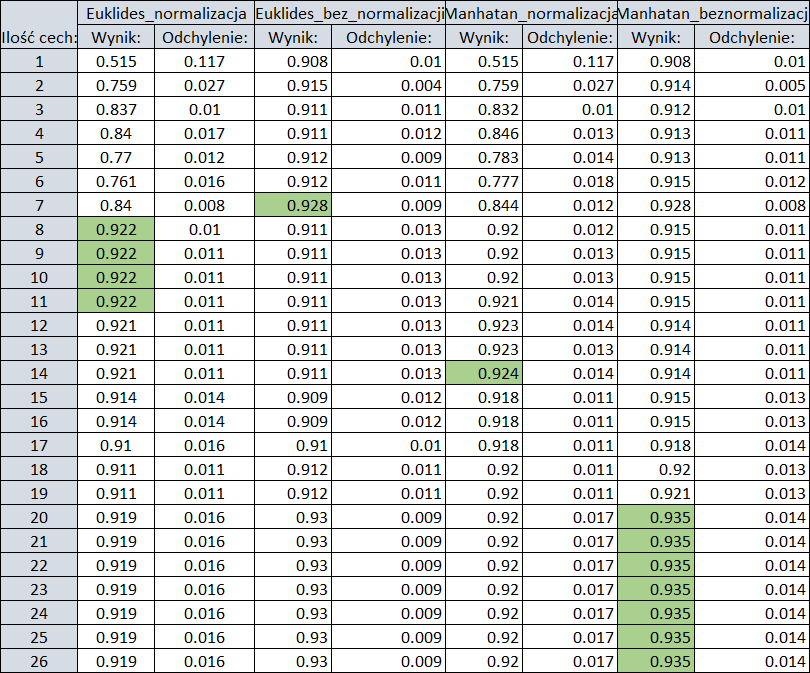
\includegraphics[scale=0.77]{images/distance_metrics/distance_metrics_tab.png}
	
\end{figure}
\begin{figure}[H]
	\centering
		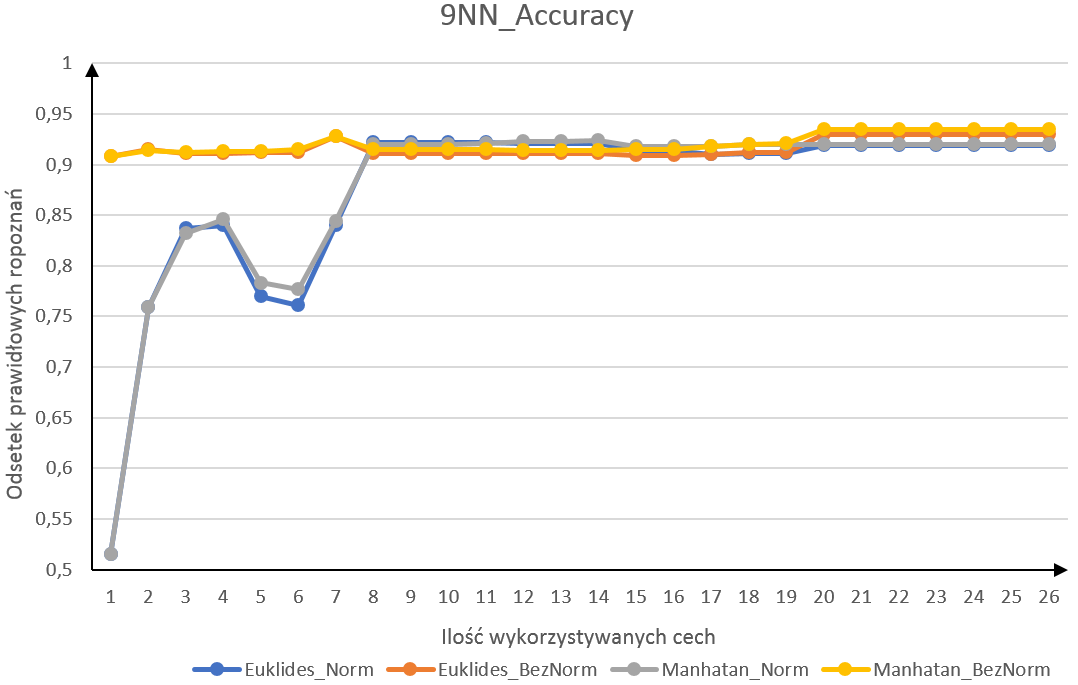
\includegraphics[scale=0.66]{images/distance_metrics/distance_metrics.png}
	\caption{Porównanie metryk odległościowych i reprezentacji wektorów cech}
	\label{odleglosci_wyk}
	
\end{figure}
\subsection{Macierz konfuzji}
\indent Poniżej przedstawiono przykładowe macierze konfuzji dla każdego z klasyfikatorów. Zgodnie z wnioskami, które przedstawiono w następnym punkcie pracy algorytmy zostały uruchomione z maksymalną wielkością wektora cech bez jego normalizacji (w tej konfiguracji uzyskiwano najlepsze wyniki). Dla każdej z macierzy poniżej znajduje się opis wyjaśniający poszczególne zależności.




%---------------------------------------------------------
%					Część szósta
%---------------------------------------------------------

\section{Dyskusja wyników i wnioski wynikające z badań.}

\indent Dla omawianego problemu rozpoznawania, analizując powyżej przedstawione tabele oraz powstałe z nich wykresy i możemy wysnuć następujące wnioski.\\
\centerline{\textbf{Metryki klasyfikacji }}\\
\indent Pierwszym parametrem poddawanym badaniom naszej analizie była metryka opisująca metodę sprawdzania poprawności wyników generowanych przez wybrany klasyfikator. Ich opis oraz wyjaśnienie działania możemy przeczytać w punkcie 4 niniejszej pracy. \\
\indent Rozpoczynając analizę, w tabeli \ref{glowna_tabela} możemy jednoznacznie zauważyć wyższość metryki accuracy nad balanced czy cohen kappa. Szczególnie niezbyt trafnym doborem dla tego problemu rozpoznawania była ostatnia z metod. Okazało się, że bardzo dobrym wynikiem w jej przypadku jest poprawność w granicach 0.8, co w porównaniu z pozostałymi metrykami wynosi zbyt mało, aby móc konkurować. \\
\indent Metoda cohen kappa osiągała bardzo słabe wyniki w przypadku normalizacji wektorów o niewielkiej liczbie cech (tabela \ref{metryki_euklides_norm_tab} lub \ref{metryki_manhatan_norm_tab}). Wydawałoby się, że metryka balanced może być najlepsza z racji niezbalansowanego zbioru danych. I faktycznie, wyniki przez nią osiągane są naprawdę bardzo dobre, jednak są minimalnie słabsze od rezultatów osiąganych przez accuracy. Obie z przytoczonych metryk zachowywały się bardzo podobnie, a ich wyniki niekiedy były prawie identyczne.\\
\indent Patrząc na wykresy znajdujące się na rysunku \ref{metryki_euklides_norm_wyk} i \ref{metryki_euklides_bnorm_wyk} możemy spostrzec różnice występujące pomiędzy znormalizowanym i nieznormalizowanym wpływem wektora na wynik. W przypadku braku normalizacji różnice pomiędzy poprawnością diagnozy dla kolejnych długości wektora nie są duże i mieszczą się w przedziale około 10\%. Najlepszy rezultat ostatecznie osiąga klasyfikator z najdłuższym wektorem cech, jednak warto zwrócić uwagę na wyróżniający się bardzo podobny wynik uzyskiwany dla ilości cech równych 7. W przypadku normalizacji sytuacja zmienia się znacząco. Najsłabsze wyniki osiągane dla najmniejszych wektorów mają poprawność rzędu 0.15 (metryka cohen cappa), natomiast najlepsze w granicach 0.92 (accuracy). Wykres różni się znacząco w porównaniu z wykorzystaniem wektora nieznormalizowanego. Wysoka wartość poprawności klasyfikatorów ustala się przy wektorze o rozmiarze 8 cech (tabela \ref{metryki_euklides_norm_tab}).  Warto jednak zauważyć, że w tym przypadku najlepszy rezultat dla każdego z algorytmu otrzymywany jest przy ilości cech w granicach 8-11, gdzie bez normalizacji dopiero  20 cech dawało najlepsze wyniki. Można zatem stwierdzić, że dzięki normalizacji możemy zaoszczędzić czas na obliczenia wykorzystywany przy wektorach o większych rozmiarach. Minusem jednak jest minimalnie mniejsza dokładność (około 1 punkt procentowy mniejsza). \\
\indent Dodatkowo warto spojrzeć na wykresy i tabele dla obu metryk odległości. Widać tam jednoznacznie, uwzględniając każdą z metryk klasyfikacji przewagę odległości manhatan (porównanie wyników zaznaczonych kolorem zielonym w tabeli \ref{metryki_euklides_bnorm_tab} i \ref{metryki_manhatan_bnorm_tab} oraz \ref{metryki_euklides_norm_tab} i \ref{metryki_manhatan_norm_tab}).\\
\centerline{\textbf{Algorytmy }}\\
\indent Wyniki osiągane przez wszystkie algorytmy nie odbiegały tak od siebie jak w przypadku metryk klasyfikacji. Ostatecznie najlepsze rezultaty zanotował klasyfikator 9 najbliższych sąsiadów, jednak nie w każdym przypadku był on najlepszy. \\
\indent Pierwszym aspektem porównania algorytmów jest normalizacja wektorów, podobnie jak w przypadku metryk klasyfikacji. W tabeli \ref{algorytmy_euklides_norm_tab} oraz \ref{algorytmy_manhatan_norm_tab} możemy porównać wyniki dla obu metryk z wykorzystaniem normalizacji wektora cech. 
Wykresy \ref{algorytmy_euklides_norm_wyk} i \ref{algorytmy_manhatan_norm_wyk} obrazujące dane z tych tabel wyglądają bardzo podobnie. Wynik algorytmów również są bardzo przybliżone. W przypadku odległości mierzonej przy pomocy  normy euklides, najskuteczniejszy był algorytm najbliższych sąsiadów z parametrem k równym 9. Maksymalne wartości osiągane były przez algorytmy dla ilości cech w granicach liczby od 8 do 16 (mniej więcej połowa wszystkich cech). Sytuacja lekko się zmienia przy normie manhatan. W tym przypadku  najlepszy jest również algorytm najbliższych sąsiadów tym razem z parametrem k wynoszącym 5. Odbiega również liczba cech, w których algorytmy osiągają maksymalne rezultaty. Dla klasyfikatorów najbliższego sąsiada jest to w przedziale od 12 do 14 cech (co nie jest znaczącą różnicą), natomiast dla algorytmu najbliższej średniej powyżej 20. Oznaczać to może, że norma manhatan nie koniecznie będzie dobra dla klasyfikatora NM. Ostatecznie minimalnie lepszy wynik udało się uzyskać dla tej właśnie metryki (różnica 0.004 punktu procentowego).\\
\indent W przypadku braku normalizacji wektora, wygląd wykresów zmienia się dość znacząco. Zmniejsza się różnica pomiędzy najlepszym a najgorszym wynikiem. Tym razem obie normy odległościowe są zgodne i w przypadku algorytmu najbliższej średniej najlepszy rezultat osiągany jest dla cech w przedziale od 2 - 5, natomiast dla algorytmu najbliżych sąsiadów dla liczby powyżej 20. W tym przypadku widać znacząco różnicę pomiędzy tymi dwoma klasyfikatorami. Różnica jest również widoczna w poprawności wykonywanych diagnoz, gdzie górą jest algorytm najbliższych sąsiadów, szczególnie z parametrem k równym 5 oraz 9. Jak ustaliliśmy już w wcześniejszych rozważaniach normalizacja może znacząco skrócić ilość wykonywanych obliczeń, o ile wcześniej będziemy znali optymalną wielkość wektora cech. Odwrotnie natomiast działa algorytm najbliższej średniej, który bez normalizacji wektora potrzebuje o wiele mniejszej liczby cech, aby uzyskać maksymalny wynik (dodatkowo jest on lepszy, tabela \ref{algorytmy_euklides_norm_tab} i \ref{algorytmy_manhatan_norm_tab}). \\
\indent Algorytm najbliższej średniej osiąga nieco słabsze wyniki klasyfikacji. Natomiast w porównaniu z algorytmem najbliższych sąsiadów jest on znacznie mniej złożony obliczeniowo, co w niektórych przypadkach może być kluczowym czynnikiem przy jego wyborze. Najsłabiej wypadał klasyfikator NN z wartością parametru k równa 1. W przypadku wielkości sąsiedztwa 5 i 9 wyniki były bardzo podobne, jednak minimalnie lepszy okazał się algorytm z k=9.\\
\centerline{\textbf{Metryki odległości i postać wektora cech}}\\
\indent Wyniki zostały przedstawione dla najlepiej działającego algorytmu w tabeli \ref{odleglosci_tab}. Można jednoznacznie stwierdzić, że przy normalizacji wektora cech nie są osiągane tak dobre wyniki jak bez normalizacji. Dokładniejsze rozważania na ten temat opisane są wyżej przy porównywaniu innych parametrów. Najlepiej dla tego klasyfikatora spisywała się norma manhatan bez normalizacji, jednak długość wektora cech(powyżej 20) musiała być znacząco większa niż w przypadku metryki euklides (8-12). Różnica najlepszych wyników pomiędzy obiema normami sięga nawet 1,3 punktu procentowego. Jest to dość dużo w porównaniu z oszczędnością czasu jaką moglibyśmy uzyskać zmniejszając wektor.

\newpage
\renewcommand\refname{Bibliografia}
\addcontentsline{toc}{section}{Bibliografia} %utworzenie w spisie treści pozycji Bibliografia
\begin{thebibliography}{9}

\bibitem{bib1}  https://en.wikipedia.org/wiki/Nearest\_centroid\_classifier

[Dostęp: 10.05.2019]

\bibitem{bib2}  https://www.researchgate.net/figure/Schematic-diagram-illustrating-the-classification-of-pixel-4-using-minimum-distance\_fig3\_294596525

[Dostęp: 10.05.2019]

\bibitem{bib3}  https://www.researchgate.net/figure/K-nearest-neighbor-classifier-KNN-for-k-1-und-k-3\_fig6\_224345777

[Dostęp: 10.05.2019]

\bibitem{bib4}  https://scikit-learn.org/stable/modules/model\_evaluation.html

[Dostęp: 11.05.2019]

\end{thebibliography}

\end{document}


